\chapter{protocol}

	The commitment tree is a tree where each vertex has an associated label representing the data that is passed on to its parent. The messages have the following format: 
	\textit{MESSAGE}
	\newline
	
	\begin{tabular}{ | l | l | l | l |}
		\hline
		ID & COUNT & VALUE & COMMITMENT \\
		\hline
		20 bits & 21 bits & 20 bits & 256 bits\\
		\hline
	\end{tabular}
	\newline
	\newline
	\textit{SIGNATURE (MESSAGE)}
	\newline

	\begin{tabular}{ |l| }
		\hline
		Encryption$_{secret-key_{node}}$( HASH ( MESSAGE ) )\\
		\hline
		500 bits\\
		\hline
	\end{tabular}
	\newline
	\newline
	\textit{CERTIFICATES}
	\newline

	\begin{tabular}{ | l | l | l | }
		\hline
			Public key  & Signature & ID \\
		\hline
			1000 bits & 500 bits & 20 bits \\
		\hline

	\end{tabular}

	\newpage

\section{Aggregation-Commit Phase}
	In this phase, the network constructs a commitment structure. 
	First, the sensor nodes at the highest depth in the aggregation tree (leaf nodes) send their \payloads,defined according to \ref{def:ct}, to their parents in the aggregation tree.
	Each internal sensor node in the aggregation tree performs an aggregation operation whenever it receives \payloads from all of its children.
	Whenever a sensor node performs an aggregation operation, it creates a commitment to the set of inputs used to compute the aggregate by computing a hash over all the inputs (including the commitments that were computed by its children). 
	Both the aggregation result and the commitment creates a payload for the aggregator.
	Then the payload, with the signature of the payload signed by the sensor node are passed on to the parent of the sensor node.
	Once the final \payloads and the signatures of those \payloads are sent to the querier, if an adversary tries to claim a different aggregation structure it gets caught.
	Our algorithm generates perfectly balanced binary trees to create commitment forests which saves the bandwidth in the verification phase compared to other approaches.

	\begin{definition}\cite{chan2006secure}\label{def:ct}
		A \textbf{\textit{commitment tree}} is a logical tree build on top of an \textbf{\textit{aggregation tree}} where each vertex has an associated \payload to it, representing data being passed on to its parent. The \payload has the following format:

		$\{id, count, value, commitment\}$\\
		Where $id$ is the unique id of the node; $count$ is the number of leaf vertices in the subtree rooted at this vertex; $value$ is the aggregate computed over all the leaves rooted in the subtree; and commitment is the cryptographic commitment.

	\end{definition}

	Our \payload format is different than the label format in \cite{chan2006secure}.
	The \payload format adds an ID field and removes the complement field from the label. 
	Our protocol helps detecting an adversary, to achieve this we send the signature of the \payload. 
	And to verify the signatures, the verifier needs the ID of that node.
	The complement field was used to verify the upper bound on the aggregation result by the \q.
	We can achieve the same result with count so sending complement was redundant and no longer required.     

	There is one leaf vertex $v_{s}$ for each sensor node $s$ with the \payload,
	\begin{equation}
		p_{s} = \{ s.id, 1,s.value, Hash( N\ ||\  s.id\ ||\  1\  ||\  s.value ) \} 
	\end{equation}
	where $N$ is the query nonce which is disseminated with each query.

	Internal vertices represent aggregation operations, and have \payloads that are defined based on their children. Suppose an internal vertex has child vertices $v_{1}, v_{2},\dotsc, v_{q}$ with the following \payloads: $p_{1}, p_{2},\dotsc, p_{q}$, where
	\begin{equation}\label{def:internal-vertice}
		p_{i} = \{ i.id, i.count, i.value, i.commitment\}
	\end{equation}
	Then the internal vertex has payload 
	\begin{equation}
		p_{s} = \{ id, count, value, commitment \} 
	\end{equation}
	\begin{equation}
		id = s.id 
	\end{equation}	
	\begin{equation}
		count = \sum{i.count}		
	\end{equation}
	\begin{equation}
		value = \sum{i.value}		
	\end{equation}
	\begin{equation}
		commitment = H (N\ ||  id\ ||  count\ ||  value\ || p_{1}\ ||\ p_{2}\ || \dotsb ||\ p_{q})		
	\end{equation}

	\textcolor{red}{Talk about signatures of the \payloads.}
	
	We use the collision resistant hash function so it's impossible for an adversary to tamper any of the commitments once they are created.

	There is a mapping between the vertices in the commitment tree and the sensor nodes in the aggregation tree, a vertex is a logical element while a node is a physical device.
	To avoid confusion, we use the term vertex for the members in the commitment tree and node for the members of the aggregation tree.
	
	% \textit{\textbf{Write about off-path values also about forests }}

	The \at is a rooted tree created from the network graph. To create an optimal \at from the given network graph is outside the scope of this thesis. Our algorithm takes any arbitrary \at as an input. One possible \at for given network graph in Figure \ref{fig:ng}is shown in the Figure \ref{fig:at}.

	We use the term \bs\  for the trusted third party. In Figure \ref{fig:at} $BS$ is the \bs.
		
	\begin{figure}[hp]
		\centering
		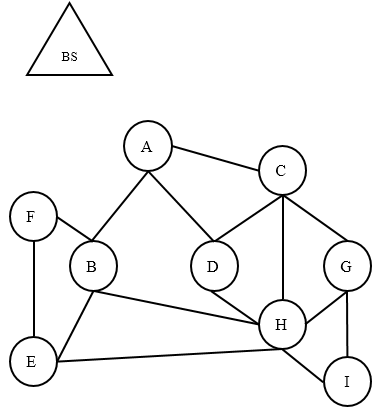
\includegraphics[scale = 0.6]{images/network-graph.png}\\
		\caption{Network graph}
		\label{fig:ng}
	\end{figure}

	\begin{figure}[hp]
		\centering
		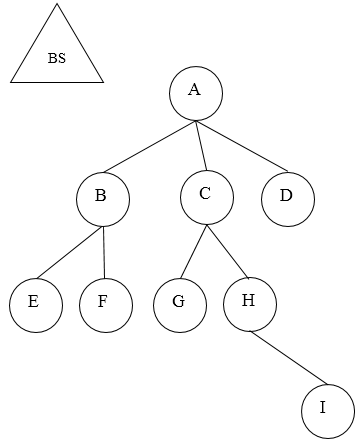
\includegraphics[scale = 0.6]{images/aggregation-tree.png}\\
		\caption{Aggregation tree for network graph in figure \ref{fig:ng}}
		\label{fig:at}
	\end{figure}

	Each sensor node $s$ has it's own sensor reading $s.value$. The querier is interested in overall behavior of the network, which is some function $f$ of all those sensor readings.
	\begin{equation}
		f(s_{1}.value, s_{2}.value, s_{3}.value, \dotsc, s_{n}.value)
	\end{equation}
	We discuss the case for the $SUM$ function, but the protocols discussed here can be applied to any other function with little or no modification. 
	\begin{equation}
		SUM = \sum\limits_{i=1}^n s_{i}.value
	\end{equation}

	\subsection{No aggregation}
		One way to calculate the $SUM$ is to send all the $n$ \payloads to the \q.
		It means all the internal nodes in the network send all the \payloads received from their descendants to their parent.
		Once the \q has all $n$ \payloads, it computes the summation.
		For any given node, the \inforate is 1. \inforate is defined in \ref{def:ir}.\\
		Advantages:
		\begin{itemize}
			\item Perfectly secure.
		\end{itemize}
		Disadvantages:
		\begin{itemize}
			\item Requires $O(n)$ bandwidth between the \bs and the \q.
			\item Requires $O(d)$ bandwidth between the internal node and its parent, where $d$ is the number of descendants for a given node.
			\item Very high \inforate.
		\end{itemize}
			
	\begin{definition}\label{def:ir}
		The \inforate for a particular node is the \payloads ratio, (number of \payloads sent) / (number of \payloads received ).
	\end{definition}

	\subsection{Naive approach}
		Another way to calculate the $SUM$ is to send only one \payload to the \q.
		It means all the internal nodes in the network, after receiving readings from all of their children, does the summation including their own reading and then pass the resulted \payload to their parents' as shown in figure NA.
		For any given node, the \inforate is $1 / (c + 1)$, where $c$ is the number of children for the give node.\\
		Advantages:
			\begin{itemize}
				\item Optimal \inforate.
			\end{itemize}
		Disadvantages:
			\begin{itemize}
				\item Makes aggregated value more vulnerable to various security attacks.
				\item Requires more bandwidth in the verification phase.
			\end{itemize}

	\subsection{Aggregate-commit approach}
		The no aggregation and naive approaches are two extreme approaches.
		The aggregate-commit approach of \cite{chan2006secure} is between these two extreme cases. It combines the advantages of both those two extreme approaches.

		In the naive approach, each sensor node $s$ sends to its parent a single message containing the \payload of the root vertex of its commitment subtree $T_{s}$.
		In the aggregate-commit approach, each sensor node $s$ sends the \payloads of the root vertices of a set of commitment subtrees $F = \{ T_{1},T_{2},\dotsc,T_{q} \} $, called commitment forest. 

		\begin{definition}\cite{chan2006secure}
			A commitment forest is a set of complete binary commitment trees such that there is	at most one commitment tree of any given height.
		\end{definition}

		We claim that the binary representation of a number $x$ illustrates the forest decomposition of the sensor node $s$, where $x$ = $1\ +$ number of descendants of $s$.
		For example, if sensor node $s$ has $22$ descendants then $x =23$, $(x)_{10}$ = $(10111)_{2}$. 
		It means $s$ has four binary trees in its outgoing forest, with the height of four, two, one and zero.
		Also, all trees in the commitment forest are complete binary and no two trees have the same height.

		The commitment forest with $n$ leaf vertices has the following properties:
		\begin{itemize}
			\item The tallest tree in the forest has height at most $\log(n)$.
			\item There are at most $\log(n)$ trees in the forest
		\end{itemize}
		In the following section we describe how to build commitment forest with an example and also how to reason about commitment forest using binary addition. 

		% It means all the internal nodes in the network pass $\log(d + 1)$ \payloads to their parents after doing the aggregation (summation), where $d$ is the number of descendants for the given node. 
		% For any given node in the network, the information rate is $\log(d+1)/(d+1)$.
		% This approach is explained in detail in the following section.     

	\subsection{Commitment Forest Generation}
		The sensor nodes at the highest depth in the aggregation tree (leaf nodes) initiate a single-vertex commitment forest, which they transmit to their parent sensor node.
		Each internal sensor node $s$ initiates a similar single-vertex commitment forest.
		In addition, $s$ also receives commitment forests from each of its children.
		Sensor node $s$ keeps track of which root vertices are received from which of its children.
		It then aggregates all the forests to form a new forest as follows.
		
		Suppose $s$ wishes to combine $q$ commitment forests $F_{1}$, $\dotsc$, $F_{q}$ and create an aggregated forest $F$.
		To do so, the sensor node $s$ merges trees with the same height in its forests, and creates a new tree with the height incremented by $1$. 
		It repeats this process until no two trees in its forest have the same height. 
		Let $T_{1}, T_{2}$ have the height $h$, where $h$ is the smallest height in $F$.
		The sensor node $s$ merges $T_{1} \& T_{2}$ into a tree of height $h + 1$ by creating a new vertex according to equation \ref{def:internal-vertice}.
		It repeats this process until all the trees have unique height in the forest.Figure \textcolor{red}{refer} shows an example of commitment forest generation process for node $A$ in Figure \ref{fig:at}.


	\newpage
	\begin{figure}[hp]
		\centering
		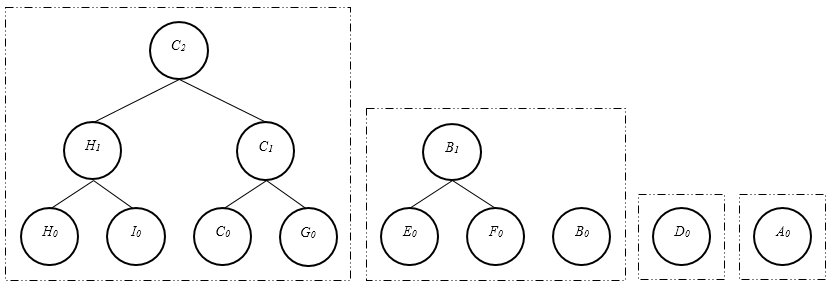
\includegraphics[scale = 0.7]{images/commitment-tree-example-1.png}\\
		\caption{NA}

		The sensor node $A$ receives the following \payloads:

		\begin{equation}
			A_{0} = \{\ A.id,\ 1,\ A.value,\ H  (\ N\ ||\ A.id\ ||\ 1\ ||\ A.value)\ \}\ (internal)
		\end{equation}
		\begin{equation}
			D_{0} = \{\ D.id,\ 1,\ D.value,\ H(\ N\ ||\ D.id\ ||\ 1\ ||\ D.value)\ \}\ (from\ D)
		\end{equation}
		\begin{equation}
			B_{0} = \{\ B.id,\ 1,\ B.value,\ H(\ N\ ||\ B.id\ ||\ 1\ ||\ B.value)\ \}\ (from\ B)
		\end{equation}
		\begin{equation}
			B_{1} = \{\ B.id,\ 2,\ B_{1}.value,\ H(\ N\ ||\ B.id\ ||\ 2\ ||\ B_{1}.value)\ \}\ (from\ B)
		\end{equation}
		\begin{equation}
			C_{2} = \{\ C.id,\ 4,\ C_{2}.value,\ H(\ N\ ||\ C.id\ ||\ 4\ ||\ C_{2}.value)\ \}\ (from\ C)
		\end{equation}
		
	\end{figure}
	
	\begin{figure}[hp]
		\centering
		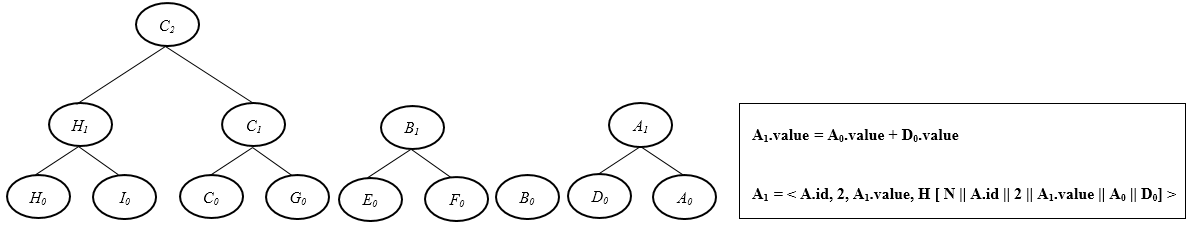
\includegraphics[scale = 0.7]{images/commitment-tree-example-2.png}\\
		\caption{First Merge: $A_{1}$ vertex created by A}
		\begin{equation}
			A_{1} = \{\ A.id,\ 2,\ A_{1}.value,\ H(\ N\ ||\ A.id\ ||\ 2\ ||\ A{1}.value\ )\ \}
		\end{equation}
		\begin{equation}
			A_{1}.value = A.value + D.value
		\end{equation}
	\end{figure}

	\begin{equation}
		A_{2} = \{\ A.id,\ 4,\ A_{2}.value,\ H(\ N\ ||\ A.id\ ||\ 4\ ||\ A{2}.value\ )\ \} 
	\end{equation}
	\begin{equation}
		A_{2}.value = A_{1}.value + B_{1}.value
	\end{equation}

	\begin{equation}
		A_{3} = \{\ A.id,\ 8,\ A_{3}.value,\ H(\ N\ ||\ A.id\ ||\ 8\ ||\ A{3}.value\ )\ \} 
	\end{equation}
	\begin{equation}
		A_{3}.value = A_{2}.value + C_{2}.value
	\end{equation}

	\textit{\textbf{ Aggregation using binary representation}}
	\[ 
		\begin{array}{lcccc}
			\mbox{Carry} & 0 & 1 & 1 & 0\\
			\hline
			\mbox{B's forest} & 0 & 0 & 0 & 1 \\
			\mbox{ } & 0 & 0 & 1 & 0 \\
			\hline
			\mbox{C's forest} & 0 & 1 & 0 & 0 \\
			\hline
			\mbox{D's forest} & 0 & 0 & 0 & 1 \\
			\hline
			\mbox{A's payload} & 0 & 0 & 0 & 1 \\
			\hline
			\mbox{Aggregation} & 1 & 0 & 0 & 1 
		\end{array}
	\] 

	\subsection{aggregator centric Aggregation-Commit approach}


\newpage
\begin{algorithm}[H]\label{number3} \caption {CommitmentTreeGeneration}
	\begin {algorithmic}[1]

		\STATE depth = \at.MaxDepth
		\WHILE {depth $\geq$ 0}

			\FORALL {\node \   $\in$ \at.depth }

			\STATE \node.\forest = NULL
					\STATE Create (\node.\msg, \sign $_{\cal{N}}$(\node.\msg))
					\STATE Attach (\node.\msg, \sign $_{\cal{N}}$(\node.\msg)) to \node.\forest
					
					\IF {\node.\children \ $\neq$ \ 0}

						\FORALL {\child \ $\in$ \node.\children }

							\FORALL {tree root \treeRoot \ $\in$ \child.\forest}

								\IF {\node \ has \treeRoot.\cert (else get \treeRoot.\cert )} 

									\IF {\node verifies \treeRoot.msg (else raise an alarm)}

										\STATE Add \treeRoot \ to \node.\forest
										
									\ENDIF
								
								\ENDIF

							\ENDFOR

							\STATE \node.\forest \ =	CommitmentTreeCoding ( \node.\forest \ ) 
						
						\ENDFOR
		
					\ENDIF


			\ENDFOR

			\STATE {depth = depth - 1 }

		\ENDWHILE
	\end{algorithmic}
\end{algorithm}

\begin{algorithm}[H]\caption{CommitmentTreeCoding}
	\begin{algorithmic}[1]

		\STATE \temp \ = SortLinkedList( \node.\forest \ )

		\WHILE {\temp.\nextTree \ $\neq$ \ 0}

			\IF {\temp.\height \ $\neq$ \ \temp.\nextTree.\height } 
				\STATE \temp \ = \temp.\nextTree
			\ELSE

				\STATE Create an aggregation node \aggregator 
				\STATE \aggregator.\height \ = \temp.\height \ + 1
				\STATE \aggregator.\lc \ = \temp
				\STATE \aggregator.\rc \ = \temp.\nextTree
				\STATE Insert \aggregator \ to \node.\forest
				\STATE Remove \temp
				\STATE Remove \temp.\nextTree
				\STATE \temp \ = SortLinkedList( \node.\forest \ )

			\ENDIF

		\ENDWHILE		

		\STATE return \temp

	\end{algorithmic}

\end{algorithm}

\newpage

\begin{algorithm}
\caption{Pseudo algorithm to detect a cheater}

	\begin{algorithmic}[1]

			\STATE \querier \ finds out all the \complainer$_{\mathcal{N}}$ $\in$ \at \ using a complainer detecting algorithm

			\FORALL {\complainer$_{\mathcal{N}}$}

				\STATE \querier \ gets \node$_{0}$, \sign $_{\cal{N}}$ ( \node$_{0}$ )
			
			\ENDFOR

			\STATE \querier \  finds possible \cheater \ based on \complainer$_{\mathcal{N}}$

			\FORALL {\cheater}

				\STATE \querier \  gets \node$_{\mathcal{I}}$, \sign $_{\cal{N}}$ ( \node$_{I}$ ) \cheater \  receives and sends. 
				\STATE If needed \querier \  gets \node$_{\mathcal{I}}$, \sign $_{\cal{N}}$ ( \node$_{I}$ ) of the \parent \ \cheater 
			
			\ENDFOR

			\STATE \querier \  determines the \cheater \ based on recived information

	\end{algorithmic}
\end{algorithm}

\textit{Properties of commitment tree and aggregation tree}

	If you have $O(n)$ children then you need at least $\Omega(n)$ \& at max $O(n\log(n))$ certificates.

	If you have $O(n)$ descendants then you need $\Omega(\log(n))$  \& at max $O(n\log(n))$ certificates.


\section{Advantages of this protocol}
\section{Disadvantages of this protocol}
